\subsection{Hausman Test for Random vs. Fixed Effects}

% Take $x_{it} $ fo which $\overline{x_i} = x_{it}, \forall i, t.$
Even if strict exogeneity is satisfied, the consistency of FE estimators comes at an efficiency
loss compared to the RE-GLS and POLS estimators.
This is easiest seen in the FD-transformation, in which we loose the $n$ observations pertaining to the first time period $t=1$.

The efficiency loss of the Within-estimator is somewhat more subtle.
It arises because the Within-estimator only exploits variation across time and disregards the
time-constant variation across cross-sectional units.

As a result, if the core RE assumption of $X_i$ and $\alpha_i$ being uncorrelated is indeed satisfied, 
we prefer the RE-estimators. If instead it is violated, we of course prefer the less efficient but consistent FE estimators.

\begin{theorem}[Hausman-Test]\label{Hausman-test}
    \
    
    $\mathcal{H}_0$: $\hat{\beta}_{RE-GLS} - \hat{\beta}_{FE-W} = 0$ 

    We define:
    \begin{align*}
        T_{Hausman} &= n \Bigl(\hat{\beta}_{FE} - \hat{\beta}_{RE} \Bigr)^{\prime} \Bigl( A\mathbb{V}[\hat{\beta}_{FE}] - A\mathbb{V}[\hat{\beta}_{RE}] \Bigr)^{-1} \Bigl(\hat{\beta}_{FE} - \hat{\beta}_{RE}\Bigr) \rightarrow \chi_k^2
    \end{align*}
    If $\mathcal{H}_0$ is accepted, the difference between $\hat{\beta}_{RE-GLS}$ and $\hat{\beta}_{FE-W}$ is small enough to suggest that
    both estimators are consistent. that $X_i$ and $\alpha_i$ are indeed uncorrelated, and therefore, 
    we should use the more efficient estimator $\hat{\beta}_{RE-GLS}$.

    If the test rejects this is evidence that the individual effect ui is correlated with the regressors so the random effects model is not appropriate.
\end{theorem}

% \begin{note}
%     \

%     To sum up, the FE estimators work under arbitrary correlation between the unobserved
% heterogeneity $\alpha_i$ and covariates $X_i$ , but they cannot deal with time-constant regressors and
% their consistency is paid for by an efficiency loss relative to RE estimators.

%     Most importantly, their consistency requires strict exogeneity, 
%     a much stronger assumption than contemporaneous exogeneity of covariates and error terms.
% \end{note}

\begin{remark}[Random Effects or Fixed Effects?(Hansen, 2022\cite{hansen2022econometrics})]
    \

    We have presented the random effects and fixed effects estimators of the regression coefficients.
Which should be used in practice? How should we view the difference?

    The basic distinction is that the random effects estimator requires the individual error $\tilde{\alpha}_i$ 
    to satisfy the conditional mean assumption $\mathbb{E}[\tilde{\alpha}_i | \tilde{X}_i] = 0$.
    The fixed effects estimator does not require this condition, and is robust to its violation. 
    
    In particular, the individual effect $\tilde{\alpha}_i$ can be arbitrarily correlated to the regressors.
    On the other hand the random effects estimator is efficient under random effects.

    Current econometric practice is to prefer robustness over efficiency. 
    Consequently, current practice is (nearly uniformly) to use the fixed effects estimator for linear panel data models. 
    Random effects estimators are only used in contexts where fixed effects estimation is unknown or challenging 
    (which occurs in many nonlinear models).
    
    The labels ``random effects'' and ``fixed effects'' are misleading. 
    These are labels which arose in the early literature and we are stuck with these labels today. 
    In a previous era regressors were viewed as ``fixed''. 
    Viewing the individual effect as an unobserved regressor leads to the label of the individual effect as ``fixed''. 
    Today, we rarely refer to regressors as ``fixed'' when dealing with observational data. 
    We view all variables as random. Consequently describing $\alpha_i$ as ``fixed'' does not make much sense 
    and it is hardly a contrast with the ``random effect'' label since under either assumption $\alpha_i$ is treated as random. 
    Once again, the labels are unfortunate but the key difference is whether $\alpha_i$ is correlated with the regressors.
\end{remark}

\subsection{FE-IV Estimation}

\begin{enumerate}
    \item Contemperaneous exogeneity: $\mathbb{E}[x_{it} u_{it}] = 0, \forall t.$
    \item Strict exogeneity: $\mathbb{E}[x_{it} u_{is}] = 0, \forall t, s.$
    \item Sequential exogeneity: $\mathbb{E}[x_{it} u_{is}] = 0, \forall t, s \geq t.$
\end{enumerate}
\begin{definition}[Predetermined variables(Or Sequantial Exogeneity)]
    \

    Predetermined variables are variables that were determined prior to the current period. 
    In econometric models this implies that the current period error term is 
    uncorrelated with current and lagged values of the predetermined variable 
    but may be correlated with future values. 
    This is a weaker restriction than strict exogeneity, 
    which requires the variable to be uncorrelated with past, present, and future shocks.
\end{definition}

The models we have discussed so far have been static with no dynamic relationships.
In many economic contexts it is natural to expect that behavior and decisions are dynamic, explicitly depending
on past behavior. 

The workhorse dynamamic model in a panel framework is the $p$-th order autoregression with regressors
and a one-way error component structure(see \ref{sec:one-way error component model}).
This is:
\begin{gather}\label{eq:FE-IV base}
    y_{it} = \alpha_1 y_{i,t-1} + \cdots + \alpha_p y_{i,t-p} + x_{it}^{\prime} \beta + \alpha_i + u_{it} 
\end{gather}
where $\alpha_j$ are the autoregressive coefficients. $x_{it}$ is a $k$-vector of regressors,
$\alpha_i$ is an individual effect and $u_{it}$ is an idiosyncratic error.
It's conventional to assume that $u_{it}$ and $\alpha_i$ are mutuallt independent and
the $u_{it}$ are serially uncorrelated and mean zero.
For the present we will assume that the regressors $x_{it}$ are strictly exgenous(assumption \ref{assumption:FE-strictexogeneity}).
Currently, we focus on the AR(1) model:
\begin{gather*}
    y_{it} = \alpha_i + u_{it} + \beta_1 y_{i,t-1} + x_{it}^{\prime} \beta_{-1}
\end{gather*}
where $\beta_{-1}$ is a $k-1$ vector of coefficients on all other regressors.

\begin{definition}[Anderson and Hsiao(1981)]
    \

    Anderson and Hsiao (1982) made an important breakthrough by showing that 
    a simple instrumental variables estimator is consistent for the parameters of \ref{eq:FE-IV base}.
    he method first eliminates the individual effect $\alpha_i$ by first differencing:
    \begin{align*}
        y_{it} &= \alpha_i + x_{it}^{\prime} \beta + u_{it} \\
        &= \alpha_i + \beta_1 y_{i, t-1} + \tilde{x}_{it}^{\prime} \beta_{-1} + u_{it}  \\
        \Rightarrow \Delta y_{it} &= \beta_1 \Delta y_{i,t-1} + \Delta x_{it}^{\prime} \beta + \Delta u_{it}
    \end{align*}
    The challenge is that first-differencing induces correlation between $\Delta y_{i,t-1}$ and $\Delta u_{it}$:
    \begin{gather*}
        \mathbb{E}[\Delta y_{i,t-1} \Delta u_{it}] = \mathbb{E}\left[ (y_{i,t-1} - y_{i,t-2})(u_{it} - u_{i,t-1})\right] = -\sigma_u^2.
    \end{gather*}
    The other regressors are not correlated with $\Delta u_{it}$.
    For $s>1$, $\mathbb{E}[\Delta y_{i,t-s} \Delta u_{it}] = 0$ and $x_{it}$ is strictly exogenous $\mathbb{E}[\Delta x_{it} \Delta u_{it}] = 0.$
    The correlation between $\Delta y_{i,t-1}$and $\Delta u_{it}$ is endogeneity. 
    One solution to endogeneity is to use an instrument. 
    Anderson-Hsiao pointed out that $y_{i,t-2}$ is a valid instrument because it is correlated with $\Delta y_{i,t-1}$ yet uncorrelated with $\Delta u_{it}$.
    Under sequential exogeneity, instrument-exogeneity is satisied:
    $\mathbb{E}[y_{i,t-2} \Delta u_{it}] = \mathbb{E}[y_{i,t-2} \Delta u_{it}] - \mathbb{E}[y_{i,t-2} \Delta u_{it-1}] = 0.$

    This is the IV usign the instruments $(y_{i,t-2}, \cdots, y_{i,t-s-1})$ for $(\Delta y_{i,t-1}, \cdots, \Delta y_{i,t-s})$.
    The estimator requires $T \geq s+2.$
    
    \[\mathbb{E}[y_{is} \Delta u_{it}] = 0, \forall s\leq t-2.\]
\end{definition}

\begin{figure}[htbp!]
    \centering
    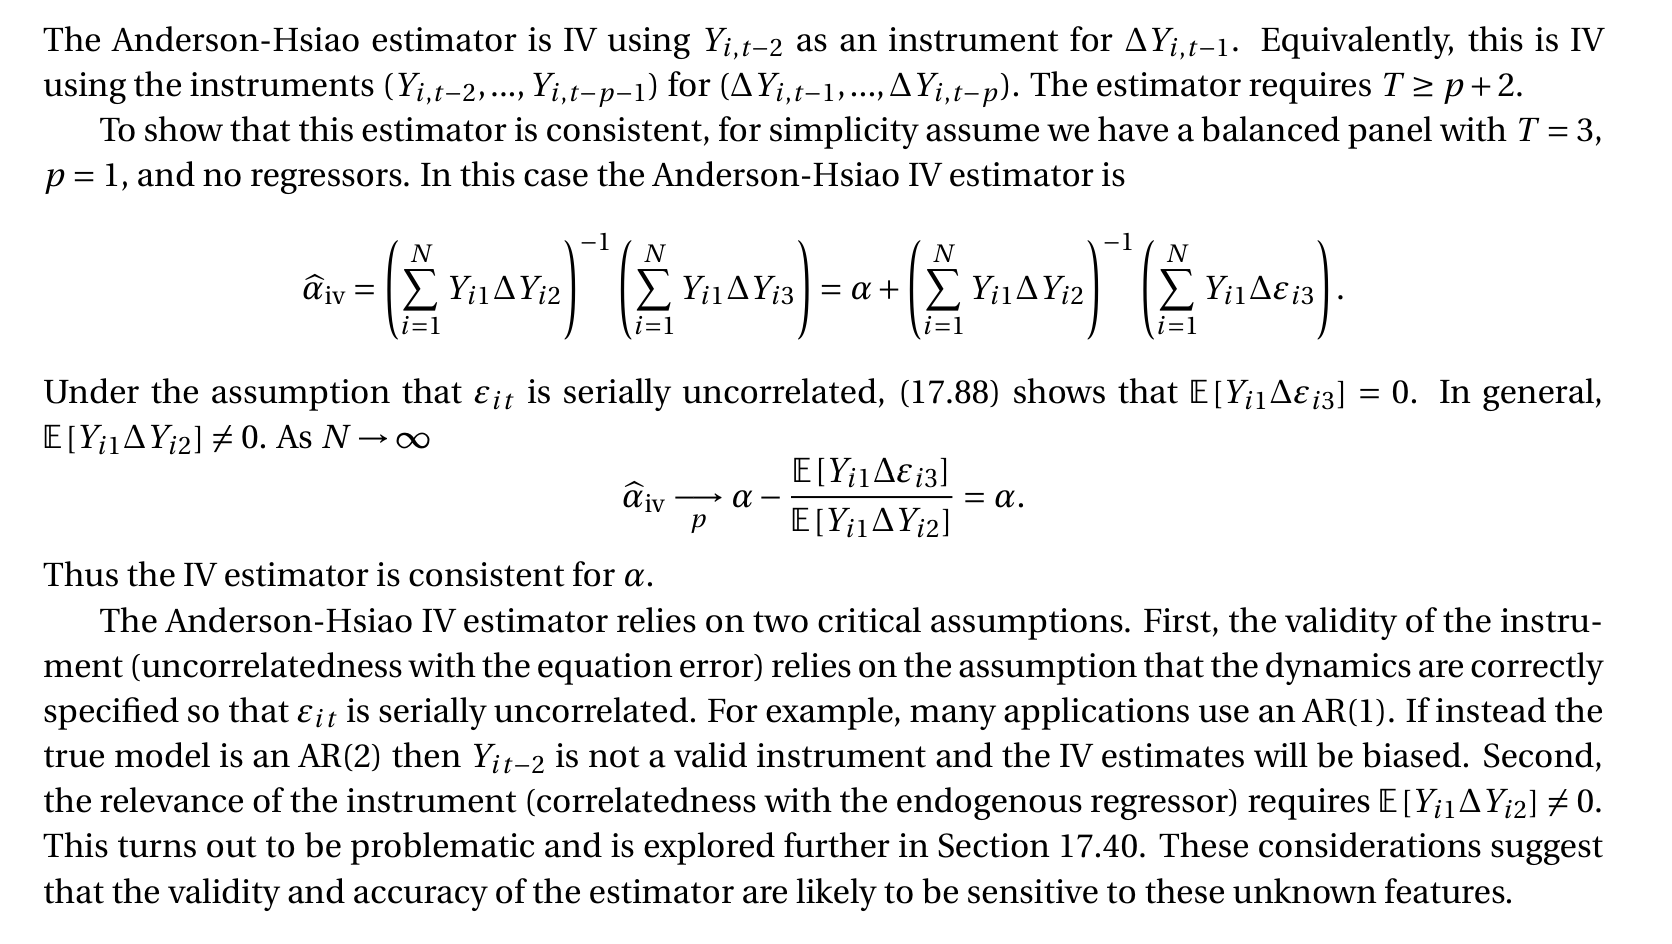
\includegraphics[width=\linewidth]{figures/Anderson-Hsiao-1981-2.png}
    \caption{Anderson and Hsiao(1981)}
\end{figure}

Using similar reasoning, other approaches use sequential exogeneity to circumvent FE methods 
altogether rather than to save their consistency. 
For example, Blundell and Bond (1998) start from the original specification:
\[y_{it} = x_{it}^{\prime} \beta + \alpha_i + u_{it}, \]
where correlation between $\alpha_{i}$ an $x_{it}$ is suspected to be due to $y_{i,t-1}$, contained in $x_{it}.$

\begin{definition}[Blundell and Bond(1998)]
    \begin{align*}
        y_{it} &= \alpha _i + \beta_1 y_{i,t-1} + u_{it} \\
        &= \beta_1 y_{i,t-1} + (u_{it} + \alpha_i) 
    \end{align*}
    Use $\Delta y_{i,t-1}$ as the IV for $y_{i,t-1}$
\end{definition}
